\documentclass[11pt, fullpage,letterpaper]{article}
\usepackage[utf8]{inputenc} % allow utf-8 input
\setlength{\parskip}{\baselineskip}%
\setlength{\parindent}{0pt}%
\usepackage[margin=1in]{geometry}

\usepackage{hyperref}       % hyperlinks
\usepackage{url}            % simple URL typesetting
\usepackage{booktabs}       % professional-quality tables
\usepackage{amsfonts}       % blackboard math symbols
\usepackage{nicefrac}       % compact symbols for 1/2, etc.
\usepackage{microtype}      % microtypography
\usepackage{xcolor}         % colors

% our imports
\usepackage{float}
\usepackage{fancyvrb}
\usepackage{algorithm}
\usepackage{algpseudocode}
\usepackage{amssymb,amsxtra,amsmath,amsthm}

\usepackage{latexsym}
\usepackage{mathtools}
\usepackage{ifthen}
\usepackage{calc,fancyhdr}
\usepackage{indentfirst}
\usepackage{parskip}
\usepackage{xurl}
\hypersetup{citecolor=DeepPink4}
\hypersetup{linkcolor=DarkRed}
\hypersetup{urlcolor=DarkBlue}
\usepackage{cleveref}

\title{A reliable implementation of the Variational Autoencoding Neural Operator (VANO)}
\author{Matthew Lowery, Ramansh Sharma}
\date{}


\begin{document}
% Math commands by Thomas Minka
\newcommand{\var}{{\rm var}}
\newcommand{\Tr}{^{\rm T}}
\newcommand{\vtrans}[2]{{#1}^{(#2)}}
\newcommand{\kron}{\otimes}
\newcommand{\schur}[2]{({#1} | {#2})}
\newcommand{\schurdet}[2]{\left| ({#1} | {#2}) \right|}
\newcommand{\had}{\circ}
\newcommand{\diag}{{\rm diag}}
\newcommand{\invdiag}{\diag^{-1}}
\newcommand{\rank}{{\rm rank}}
% careful: ``null'' is already a latex command
\newcommand{\nullsp}{{\rm null}}
\newcommand{\tr}{{\rm tr}}
\renewcommand{\vec}{{\rm vec}}
\newcommand{\vech}{{\rm vech}}
\renewcommand{\det}[1]{\left| #1 \right|}
\newcommand{\pdet}[1]{\left| #1 \right|_{+}}
\newcommand{\pinv}[1]{#1^{+}}
\newcommand{\erf}{{\rm erf}}
\newcommand{\hypergeom}[2]{{}_{#1}F_{#2}}

% boldface characters
\renewcommand{\a}{{\bf a}}
\renewcommand{\b}{{\bf b}}
\renewcommand{\c}{{\bf c}}
\renewcommand{\d}{{\rm d}}  % for derivatives
\newcommand{\e}{{\bf e}}
\newcommand{\f}{{\bf f}}
\newcommand{\g}{{\bf g}}
\newcommand{\h}{{\bf h}}
%\newcommand{\k}{{\bf k}}
% in Latex2e this must be renewcommand
\renewcommand{\k}{{\bf k}}
\newcommand{\m}{{\bf m}}
\newcommand{\mb}{{\bf m}}
\newcommand{\n}{{\bf n}}
\renewcommand{\o}{{\bf o}}
\newcommand{\p}{{\bf p}}
\newcommand{\q}{{\bf q}}
\renewcommand{\r}{{\bf r}}
\newcommand{\s}{{\bf s}}
\renewcommand{\t}{{\bf t}}
\renewcommand{\u}{{\bf u}}
\renewcommand{\v}{{\bf v}}
\newcommand{\w}{{\bf w}}
\newcommand{\x}{{\bf x}}
\newcommand{\y}{{\bf y}}
\newcommand{\z}{{\bf z}}
%s\newcommand{\l}{\boldsymbol{l}}
\newcommand{\A}{{\bf A}}
\newcommand{\B}{{\bf B}}
\newcommand{\C}{{\bf C}}
\newcommand{\D}{{\bf D}}
\newcommand{\E}{{\bf E}}
\newcommand{\F}{{\bf F}}
\newcommand{\G}{{\bf G}}
\renewcommand{\H}{{\bf H}}
\newcommand{\I}{{\bf I}}
\newcommand{\J}{{\bf J}}
\newcommand{\K}{{\bf K}}
\renewcommand{\L}{{\bf L}}
\newcommand{\M}{{\bf M}}
\newcommand{\N}{\mathcal{N}}  % for normal density
%\newcommand{\N}{{\bf N}}
\renewcommand{\O}{{\bf O}}
\renewcommand{\P}{{\bf P}}
\newcommand{\Q}{{\bf Q}}
\newcommand{\R}{{\bf R}}
\renewcommand{\S}{{\bf S}}
\newcommand{\T}{{\bf T}}
\newcommand{\U}{{\bf U}}
\newcommand{\V}{{\bf V}}
\newcommand{\W}{{\bf W}}
\newcommand{\X}{{\bf X}}
\newcommand{\Y}{{\bf Y}}
\newcommand{\Z}{{\bf Z}}

% this is for latex 2.09
% unfortunately, the result is slanted - use Latex2e instead
%\newcommand{\bfLambda}{\mbox{\boldmath$\Lambda$}}
% this is for Latex2e
\newcommand{\bfLambda}{\boldsymbol{\Lambda}}

% Yuan Qi's boldsymbol
\newcommand{\bsigma}{\boldsymbol{\sigma}}
\newcommand{\balpha}{\boldsymbol{\alpha}}
\newcommand{\bpsi}{\boldsymbol{\psi}}
\newcommand{\bphi}{\boldsymbol{\phi}}
\newcommand{\boldeta}{\boldsymbol{\eta}}
\newcommand{\Beta}{\boldsymbol{\eta}}
\newcommand{\btau}{\boldsymbol{\tau}}
\newcommand{\bvarphi}{\boldsymbol{\varphi}}
\newcommand{\bzeta}{\boldsymbol{\zeta}}

\newcommand{\blambda}{\boldsymbol{\lambda}}
\newcommand{\bLambda}{\mathbf{\Lambda}}
\newcommand{\bOmega}{\mathbf{\Omega}}
\newcommand{\bomega}{\mathbf{\omega}}
\newcommand{\bPi}{\mathbf{\Pi}}

\newcommand{\btheta}{\boldsymbol{\theta}}
\newcommand{\bpi}{\boldsymbol{\pi}}
\newcommand{\bxi}{\boldsymbol{\xi}}
\newcommand{\bSigma}{\boldsymbol{\Sigma}}

\newcommand{\bgamma}{\boldsymbol{\gamma}}
\newcommand{\bGamma}{\mathbf{\Gamma}}

\newcommand{\bmu}{\boldsymbol{\mu}}
\newcommand{\1}{{\bf 1}}
\newcommand{\0}{{\bf 0}}

% \newcommand{\comment}[1]{}

\newcommand{\bs}{\backslash}
\newcommand{\ben}{\begin{enumerate}}
\newcommand{\een}{\end{enumerate}}

 \newcommand{\notS}{{\backslash S}}
 \newcommand{\nots}{{\backslash s}}
 \newcommand{\noti}{{\backslash i}}
 \newcommand{\notj}{{\backslash j}}
 \newcommand{\nott}{\backslash t}
 \newcommand{\notone}{{\backslash 1}}
 \newcommand{\nottp}{\backslash t+1}
% \newcommand{\notz}{\backslash z}

\newcommand{\notk}{{^{\backslash k}}}
%\newcommand{\noti}{{^{\backslash i}}}
\newcommand{\notij}{{^{\backslash i,j}}}
\newcommand{\notg}{{^{\backslash g}}}
\newcommand{\wnoti}{{_{\w}^{\backslash i}}}
\newcommand{\wnotg}{{_{\w}^{\backslash g}}}
\newcommand{\vnotij}{{_{\v}^{\backslash i,j}}}
\newcommand{\vnotg}{{_{\v}^{\backslash g}}}
\newcommand{\half}{\frac{1}{2}}
\newcommand{\msgb}{m_{t \leftarrow t+1}}
\newcommand{\msgf}{m_{t \rightarrow t+1}}
\newcommand{\msgfp}{m_{t-1 \rightarrow t}}

\newcommand{\proj}[1]{{\rm proj}\negmedspace\left[#1\right]}
\newcommand{\argmin}{\operatornamewithlimits{argmin}}
\newcommand{\argmax}{\operatornamewithlimits{argmax}}

\newcommand{\dif}{\mathrm{d}}
\newcommand{\abs}[1]{\lvert#1\rvert}
\newcommand{\norm}[1]{\lVert#1\rVert}

%miscellaneous symbols
\newcommand{\ie}{{{i.e.,}}\xspace}
\newcommand{\eg}{{{\em e.g.,}}\xspace}
\newcommand{\EE}{\mathbb{E}}
\newcommand{\VV}{\mathbb{V}}
\newcommand{\sbr}[1]{\left[#1\right]}
\newcommand{\rbr}[1]{\left(#1\right)}
\newcommand{\cmt}[1]{}



\maketitle

\section{Introduction}

% Problem definition and motivation - 
% --what problem did you choose? 
% --Why is it important or interesting? 
% --Why did you use machine learning techniques to solve it?

For this final project, we chose to implement VANO, the Variational Neural Operator (VANO; \cite{seidman2023variational}). We considered it an interesting endeavor in so much as our research deals with operator learning and working with functional data, versus most ML methods that are limited to finite dimensional vectors. Additionally, VANO is a probabilistic model that performs variational inference which means it aligns itself well within the subjects covered in the Probabilistic Machine Learning class. 

VANO is first a variational autoencoder (VAE), but adapted for functional datasets, which are a new paradigm for the field of machine learning (ML). VANO learns a smooth distribution over functions that can be sampled from to generate new functions, in a \emph{generative} capacity. In addition, the latent distribution's dimensionality is reduced significantly as compared to the input, which makes a useful, compact, and accurate \textit{summary} of the functional data that is cheaper to store and use. Among many applications, one can use the latent distribution to perform anomaly detection. 

While classical methods such as k-means and PCA can encode any data, which may include function evaluations, they are not necessarily able to capture complex, physical, and non-linear relationship between the input data points. Moreover, they are far inferior to the highly-nonlinear approximation that deep learning methods is capable of. Moreover, classical methods cannot learn a probabilistic distribution which can be sampled from to generate new examples. 

We initially thought VANO was tailored to learn operators; essentially, it encodes a given input function, samples from the latent distribution and uses the decoded representation as a proxy for the output function of the operator. While VANO potentially has this capability, \textbf{it currently focuses on learning the identity operator of the functions just as standard VAEs do with feature vectors, images, and other datasets}. We utilize the model in our work in this way, taking the input functions from some of the canonical operator learning datasets and learning their underlying distribution. 

% Our goal for this project is to write a well documented codebase for this model for numerous 1D and 2D operator learning datasets (including Burgers, Advection, cavity flow, and Darcy flow) as the original work did not release any code. Borrowing notation from the paper, the encoding map $\mathcal{E}(u): u \rightarrow \mathbb{R}^n, \; u \sim \mathcal{X}$, maps an input function $u$ to a latent $n$-dimensional vector. The decoding map maps the latent space to a function $\mathcal{Y}$ that can be evaluated in its domain; $\mathcal{D}: \mathbb{R}^n \rightarrow \mathcal{Y}$.

\section{Motivation}
The operator learning problem involves learning an approximation map between a given set of input and output functions \cite{Lu_2021, fair_paper} which can then be evaluated on previously unseen examples of functions. While machine learning techniques are readily useful with a large variety of architectures for this problem, more traditional scientific computing techniques are not. Traditional techniques such as principal component analysis (PCA) and proper orthogonal decomposition (POD) are by themselves not expressive enough for large scale datasets or difficult operator learning problems (ones that involve mix of global/local information in the PDE, oscillatory problems, etc.). However, these techniques are useful in unsupervised models such as variational autoencoding neural operators (VANO) \cite{seidman2023variational}.   

Without loss of generality, we describe the operator learning problem here. Let $U=\{u_i\}_{i=0}^{N_u}$ and $V=\{v_j\}_{j=0}^{N_v}$ be two sets of functions. The operator $\tilde{G}: \mathcal{U} \rightarrow \mathcal{V}$ is the continuous operator where $u \sim \mathcal{U}$ and $v \sim \mathcal{V}$. Discretely, let $u: \mathbb{R}^{d_1} \rightarrow \mathbb{R}^{d_2}$ be an input function and $x \in \mathbb{R}^{d_1}$ and $y \in \mathbb{R}^{q}$ be points where $d_{1}, d_2, q \in \mathbb{N}$. While it is not necessarily true, the output function $v$ is usually also a map as such $v: \mathbb{R}^{d_1} \rightarrow \mathbb{R}^{d_2}$. Using a machine learning method, one then approximates the operator $G: U \rightarrow V$ by optimizing parameters with a loss function.

\section{VANO}

VANO uses a traditional VAE to learn a reconstruction representation of \textit{functional data}. It is an unsupervised machine learning model to generate high quality functional data, something that is limited in other models right now. It does so by first passing the functional data through an encoder network. This network is agnostic of any machine learning based architecture; popular choices include multilayer perceptrons (MLPs) or convolutional neural networks (CNN). Let the encoder map by denoted as $\mathcal{E}: \mathcal{U} \rightarrow \z$, where $\mathcal{X}$ is the space of the input function and $\z$ is the \textit{latent representation}. In practice, $\z$ is a finite dimensional representation; $\z \in \mathcal{R}^n$. We experiment over the same range of $n$ as \cite{vano}. The input function $u \sim \mathcal{X}$ is used at evaluated locations; $\u \sim \mathcal{U} \in \mathcal{R}^m$. To make the autoencoder variational, VAEs and VANO use the reparameterization trick to ensure that the mean and variance w.r.t. which the latent distribution are sampled are able to be backpropagated through by automatic differentiation. This is a common trick and is done as follows; given a mean $\mu$ and variance $\sigma$ (that are being learned by the model), the latent distribution is sampled from these parameters as
\begin{align}
\z = \mu + \sigma \; \epsilon,
\end{align}

where $\epsilon \sim \mathcal{N}(0, \I)$ is the standard normal distribution. In order to make sure the network does not learn the trivial variance of $0$, in addition to the standard mean squared loss for reconstruction, the Kullback-Leibler (KL) divergence term is used to regularize the latent space to make it as close to a standard normal distribution as possible. This ensures stability in the model's performance. The KL loss is added as evidence lower bound (ELBO) in the model's loss function. The sample of the latent representation $\z$ (using the reparameterization trick) is then passed to the decoder network of the architecture. This architecture is similarly unconstrained for the architecture choice as the encoder. An appropriate architecture is decided based on the sampling grid of the input and output functions. If the functions are evaluated on a regular cartesian grid, a CNN is an appropriate choice. Otherwise, a graph neural network or a standard MLP is suitable. We denote the decoder map as $\mathcal{D}: \z \rightarrow \mathcal{V}$, where $\mathcal{V}$ is the space of the output functions (in the case of VANO, it is the same space as that of the input function). Once trained, the decoder component of the network can generate new functions in the latent coordinate space which can be evaluated anywhere in their domain. We reuse Figure \ref{fig:vano}, borrowed from \cite{seidman2023variational}, which shows the encoder and decoder transformations on a function. The variational family of the latent space is chosen to be multivariate Gaussians with diagonal covariance.

Next, we describe the implementation of VANO in this project.

\subsection{Implementation}

% We have thus far implemented standard VAEs as a helpful precursor to coding VANO. In adddition, we have implementations of standard operator learning models such as DeepOnet and FNO already, which we will compare VANO against. 

In this project, we use the Jax machine learning framework \cite{jax}. While other machine learning frameworks such as PyTorch and Tensorflow exist, we pick Jax because of its superior modularity, composable functions, and functional perspective. In our \texttt{jax\_networks.py} module, we provide implementations for common machine learning modules such as linear layers, MLPs, CNNs, as well as models relevant to our work such as DeepONets. Our main implementation of the VANO architecture is in this same module. In the VANO module, we split the output of the encoder MLP into the trainable mean and log-variance components. These two are then used to sample the latent distribution with the reparameterization trick. Subsequently, the decoder is composed of two MLPs; one to encode the spatial information where the ouptut function is evaluated, and the other to encode the sampled latent distribution. The two MLP outputs are concatenated and then passed through a final decoder MLP. The loss function is implemented in the individual files for the three problems we test on; \texttt{main\_burgers.py}, \texttt{main\_darcy\_tri.py}, and \texttt{main\_advection.py}.

\subsection{GitHub}
Our code base can be found at the following github link: \url{https://github.com/mwl10/generative_nos}. 

\section{Results}

\subsection{Dataset}
\label{sec:dataset}

In this project, we work with the following three datasets taken from \cite{fair_paper}:

\begin{enumerate}
    \item Burgers:

        The one dimensional Burgers' equation with periodic boundary conditions where $\nu=0.1$ is the viscosity. The operator learning problem for VANO in this case is recovering the input function at the initial condition; $u_0(x)$.

        \begin{align}
            \frac{\partial u}{\partial t} + u \frac{\partial u}{\partial x} = \nu \frac{\partial^2 u}{\partial x^2}, x \in (0, 1), t \in (0, 1].
        \end{align}

        The initial conditions for the training set of functions are generated according to a random distribution $\mu = \mathcal{N}(0, 625(- \Delta + 25 \I)^{-2})$. The spatial resolution is done with 128 grids.

    \item Advection:

        The advection equation with periodic boundary conditions. The initial condition is chosen as a square wave. The mesh is chosen to be $40x40$ in space and time. VANO learns the initial condition $u_0(x)$.
        \begin{align}
            \frac{\partial u}{\partial t} + \frac{\partial u}{\partial x} = 0, x \in [0, 1], t \in [0, 1].
        \end{align}

    \item Darcy flow:

        Darcy flow (or variable coefficient Poisson's equation) is our final dataset. A Gaussian process is used to generate the boundary conditions for each boundary on the triangular domain.

        \begin{align}
            - \nabla \cdot (K(x, y) \nabla h(x, y)) = f, \; (x, y) \in \Omega,
        \end{align}

        where $K$ is the permeability field, $h$ is the pressure, and $f$ is a source term which can either be a constant or a space-dependent function. \textbf{Note}: Darcy flow has 4 variations, (1) rectangular domain with continuous permeability field, (2) rectangular domain with piecewise constant permeability field, (3) triangular domain, and (4) triangular domain with a notch. We use the variation with the triangular domain with no notch for our study. VANO learns the input function of the permeability field.
\end{enumerate}

\begin{figure}
    \centering
    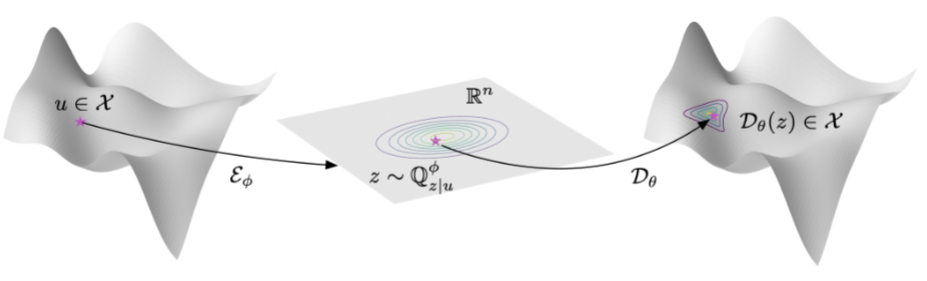
\includegraphics[width=0.5\linewidth]{fig.png}
    \caption{Figure 1 from VANO.}
    \label{fig:vano}
\end{figure}

\section{Results}
All our MLP networks are three layers wide, with 64 nodes each, using the leaky-ReLU activation function. We use the Adam optimizer to train the network with an inverse time decay learning rate schedule. The peak learning rate is chosen to be $1e-3$ with a decay rate of 0.5. We train over 50000 epochs. We go over the latent dimensions $n = [8, 16, 32]$ for our experiments.

\begin{enumerate}

\item Burgers' equation
\begin{figure}[h]
    \centering
    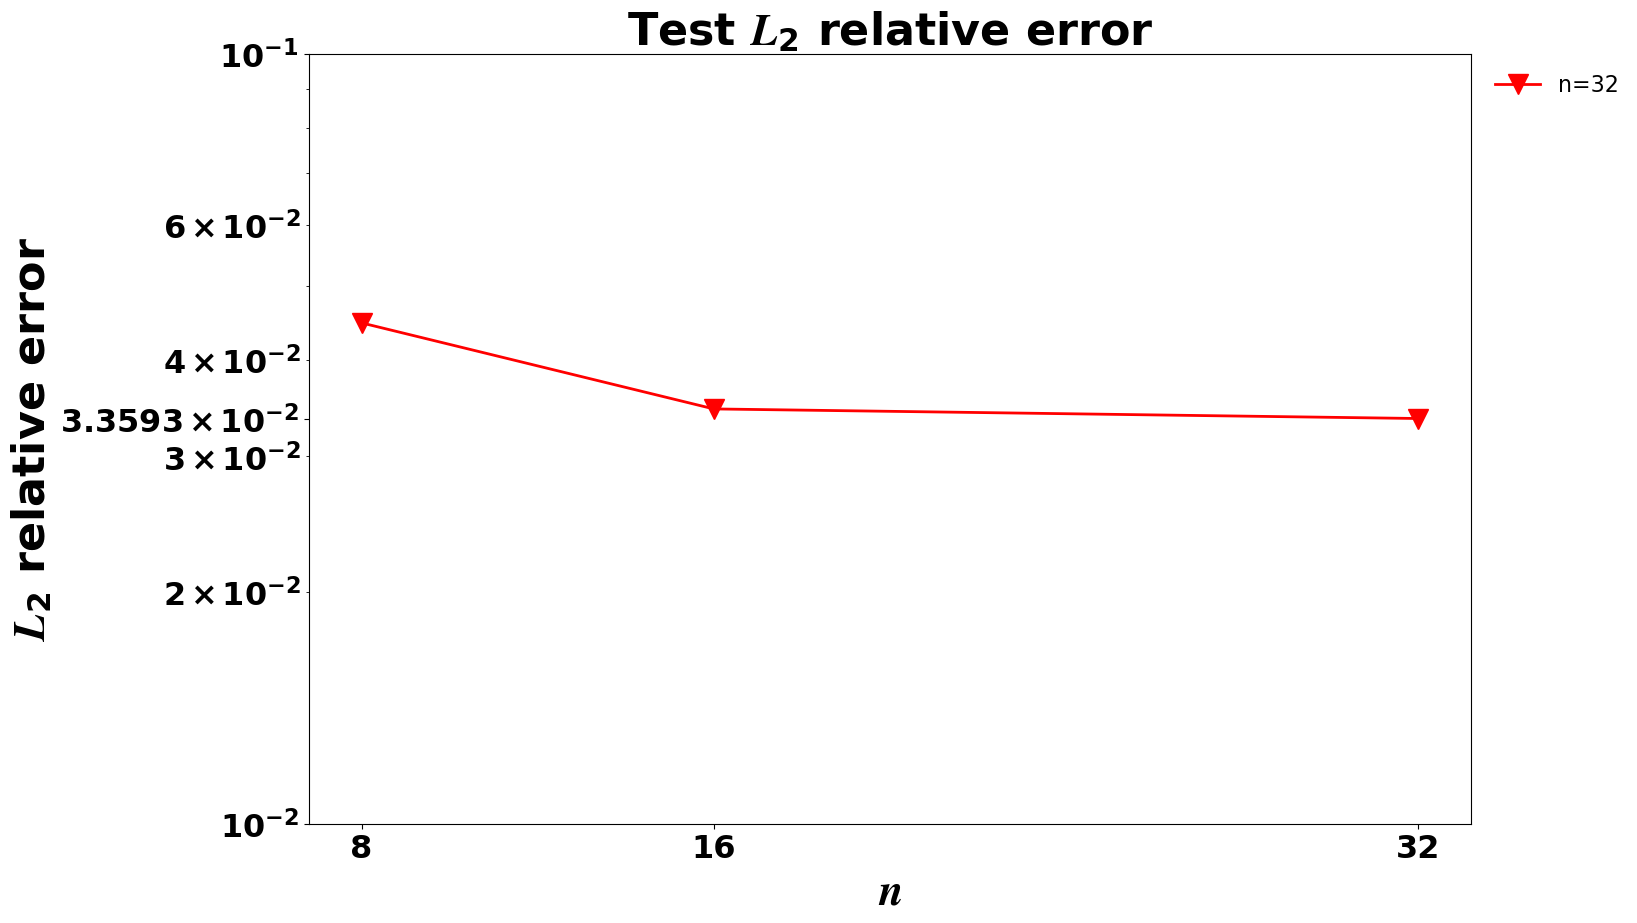
\includegraphics[width=0.5\linewidth]{all_plots/Burgers/test_l2_vs_size.png} 
    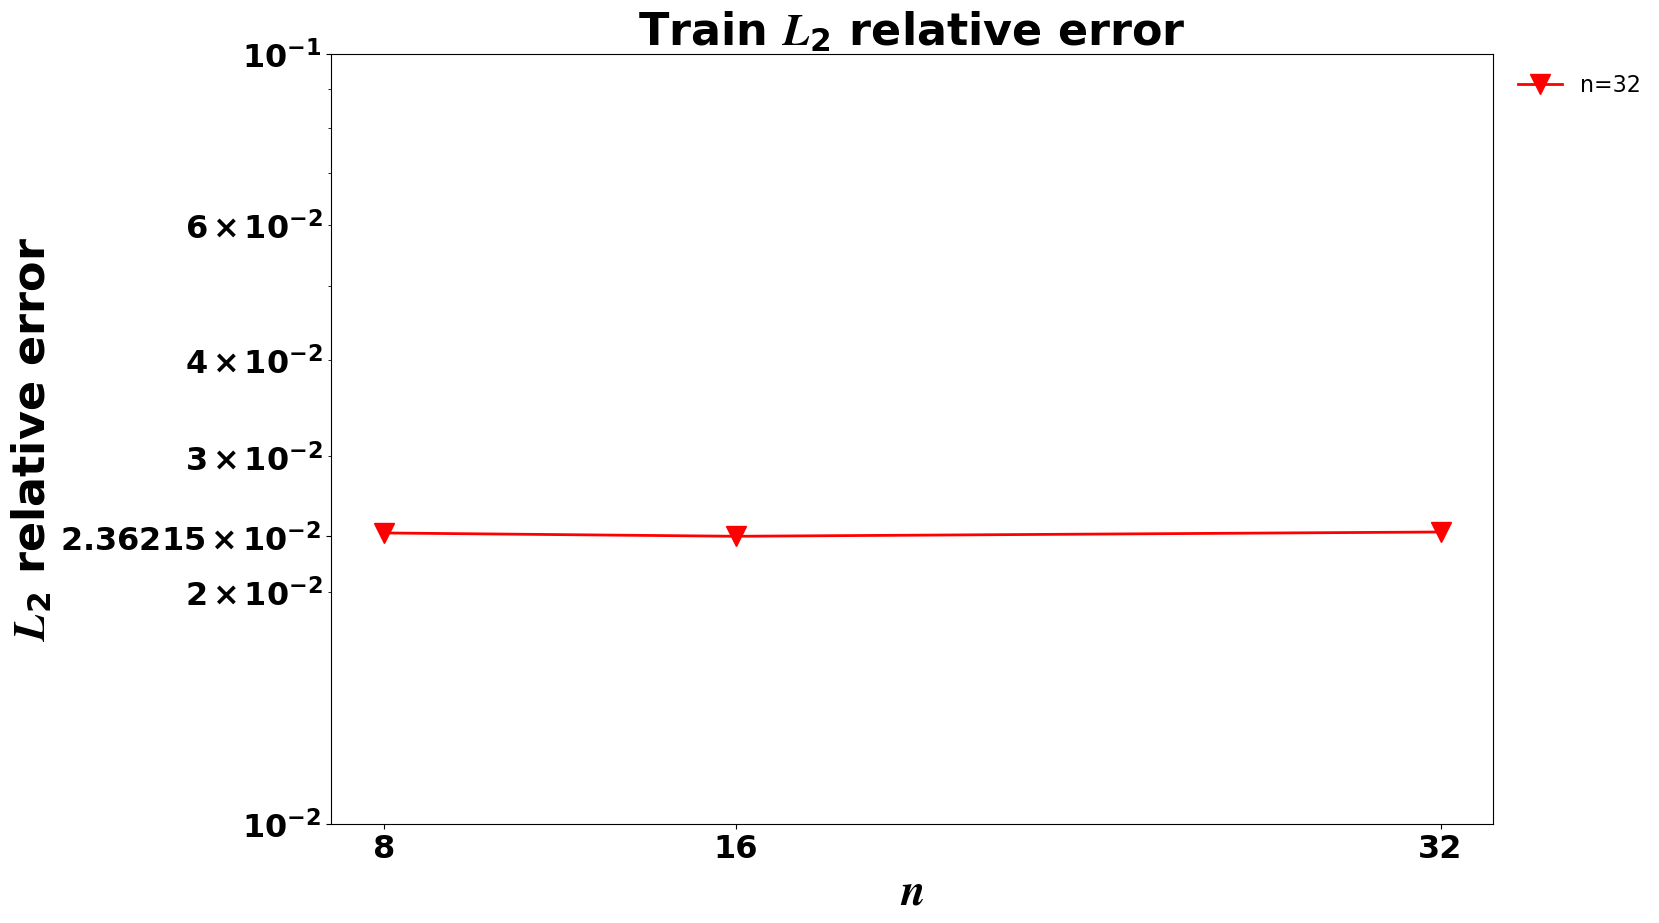
\includegraphics[width=0.5\linewidth]{all_plots/Burgers/train_l2_vs_size.png} 
    \caption{Relative $L_2$ errors on the training and test sets for the Burgers' equation.}
    \label{fig:burgers_l2}
\end{figure}

\begin{figure}[h]
    \centering
    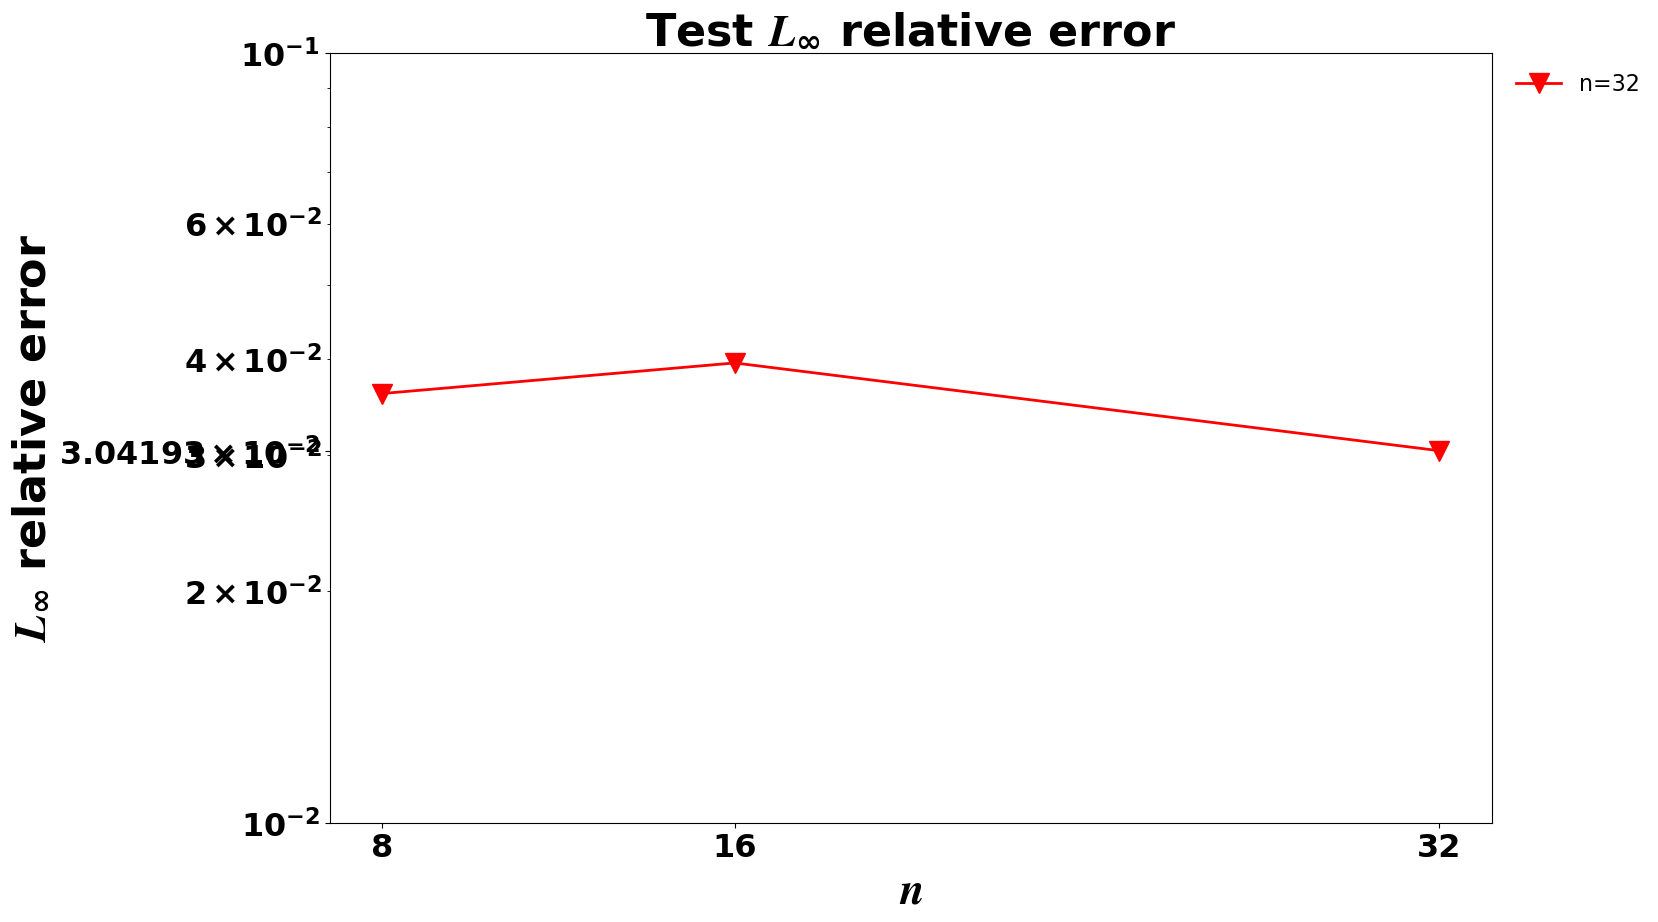
\includegraphics[width=0.5\linewidth]{all_plots/Burgers/test_linf_vs_size.png} 
    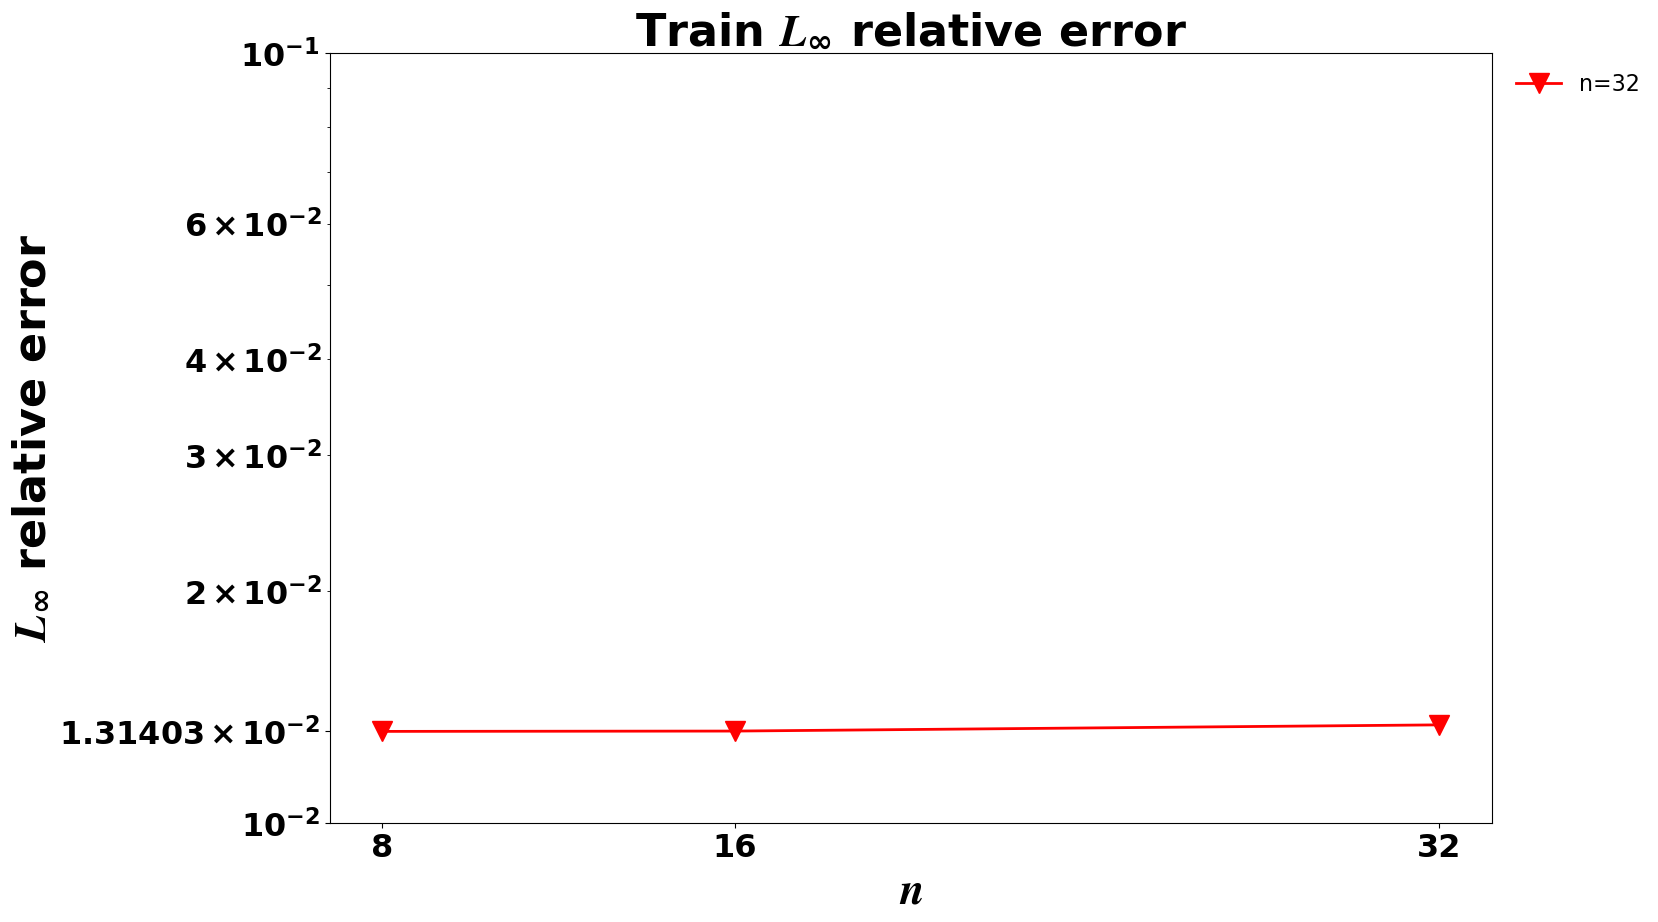
\includegraphics[width=0.5\linewidth]{all_plots/Burgers/train_linf_vs_size.png} 
    \caption{Relative $L_\infty$ errors on the training and test sets for the Burgers' equation.}
    \label{fig:burgers_linf}
\end{figure}

In Figures \ref{fig:burgers_l2} and \ref{fig:burgers_linf}, we present relative $L_2$ and $L_\infty$ results over the training and test sets for the Burgers equation.We observe that VANO achieves a low enough relative error recovering the input function, on the order of magnitude of $1e-2$. The model is also agnostic in this problem to the latent dimension used $n$. This is probably due to the problem being one-dimensional. In higher dimension, we expect a higher $n$ to approximate the function better with a richer latent distribution.

\item Advection equation

\begin{figure}[h]
    \centering
    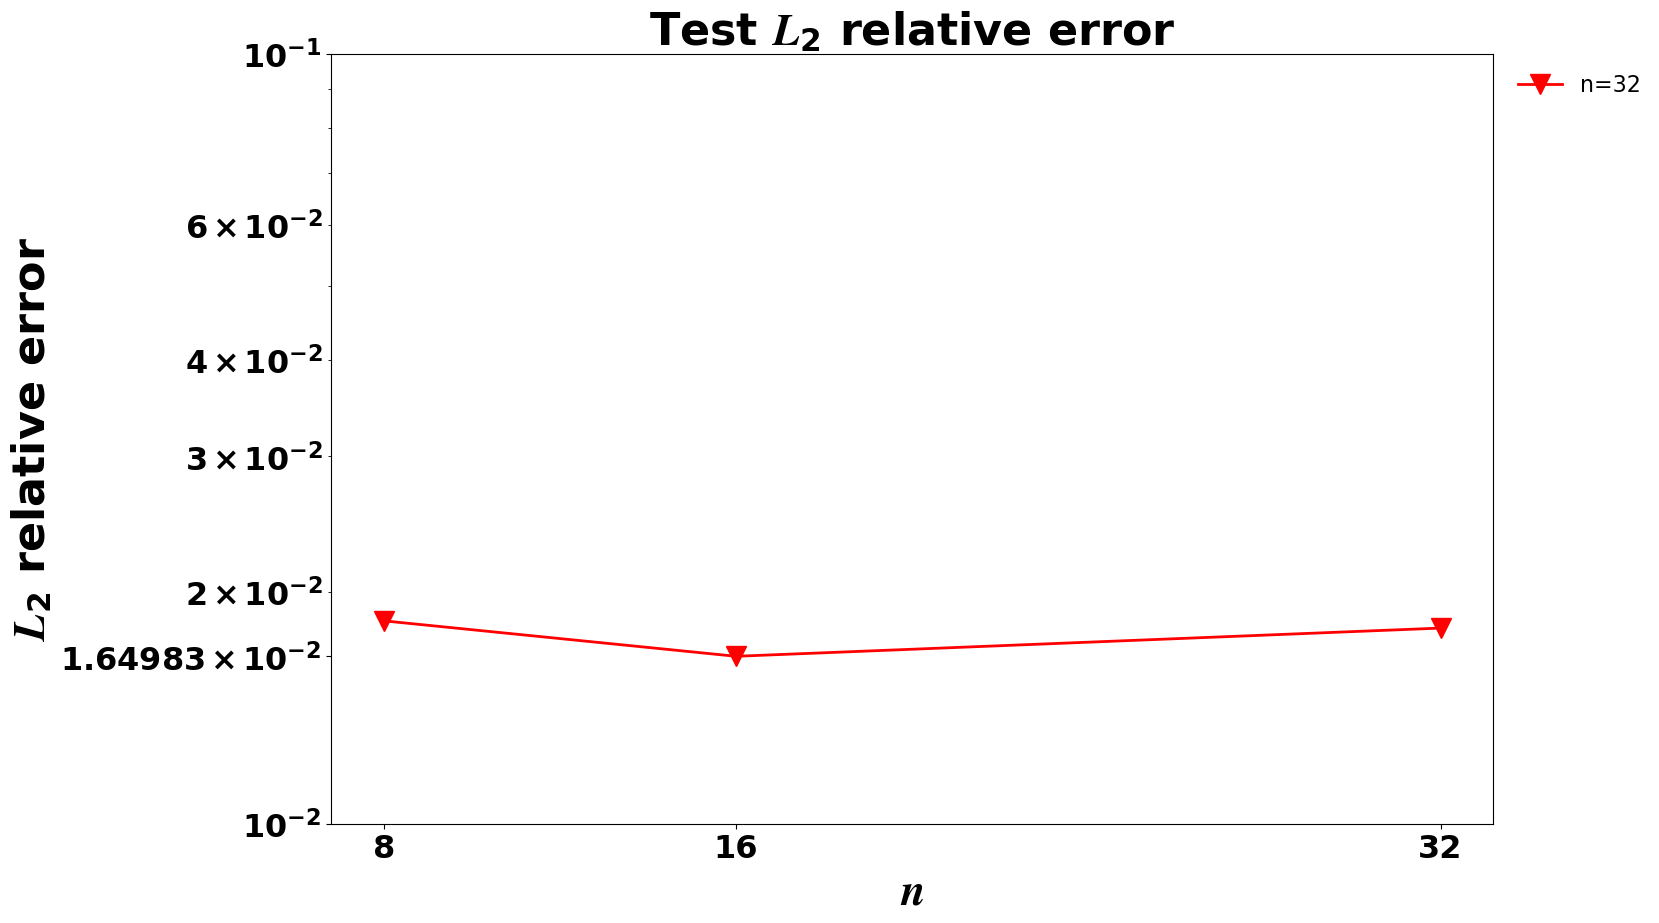
\includegraphics[width=0.5\linewidth]{all_plots/Advection/test_l2_vs_size.png} 
    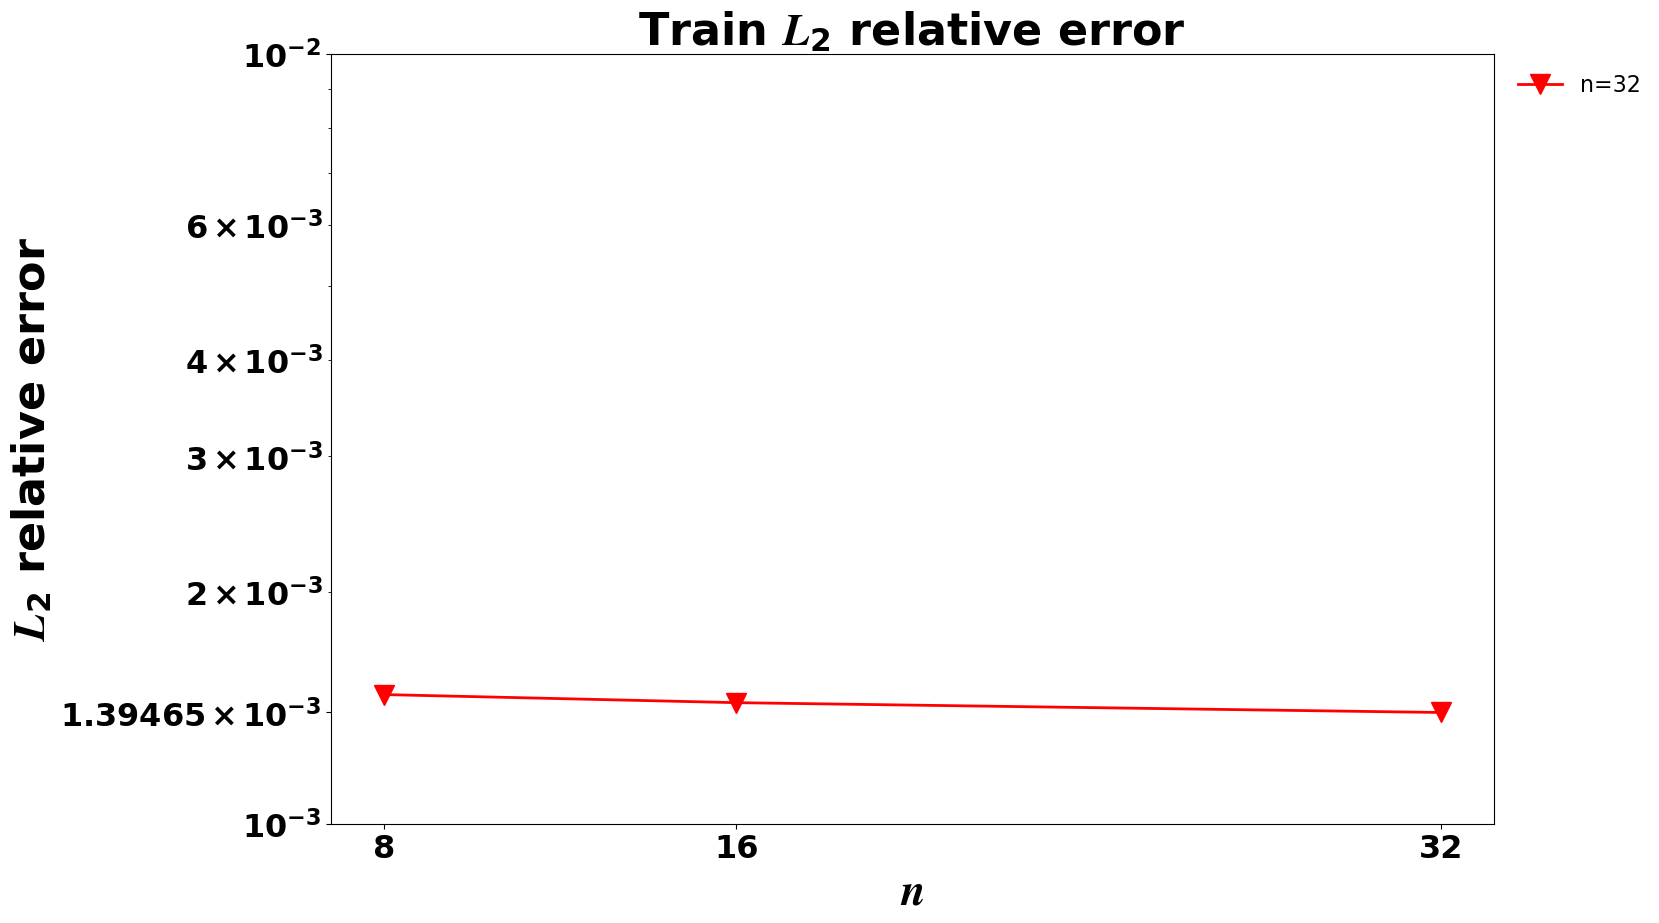
\includegraphics[width=0.5\linewidth]{all_plots/Advection/train_l2_vs_size.png} 
    \caption{Relative $L_2$ errors on the training and test sets for the Advection equation.}
    \label{fig:advection_l2}
\end{figure}

\begin{figure}[h]
    \centering
    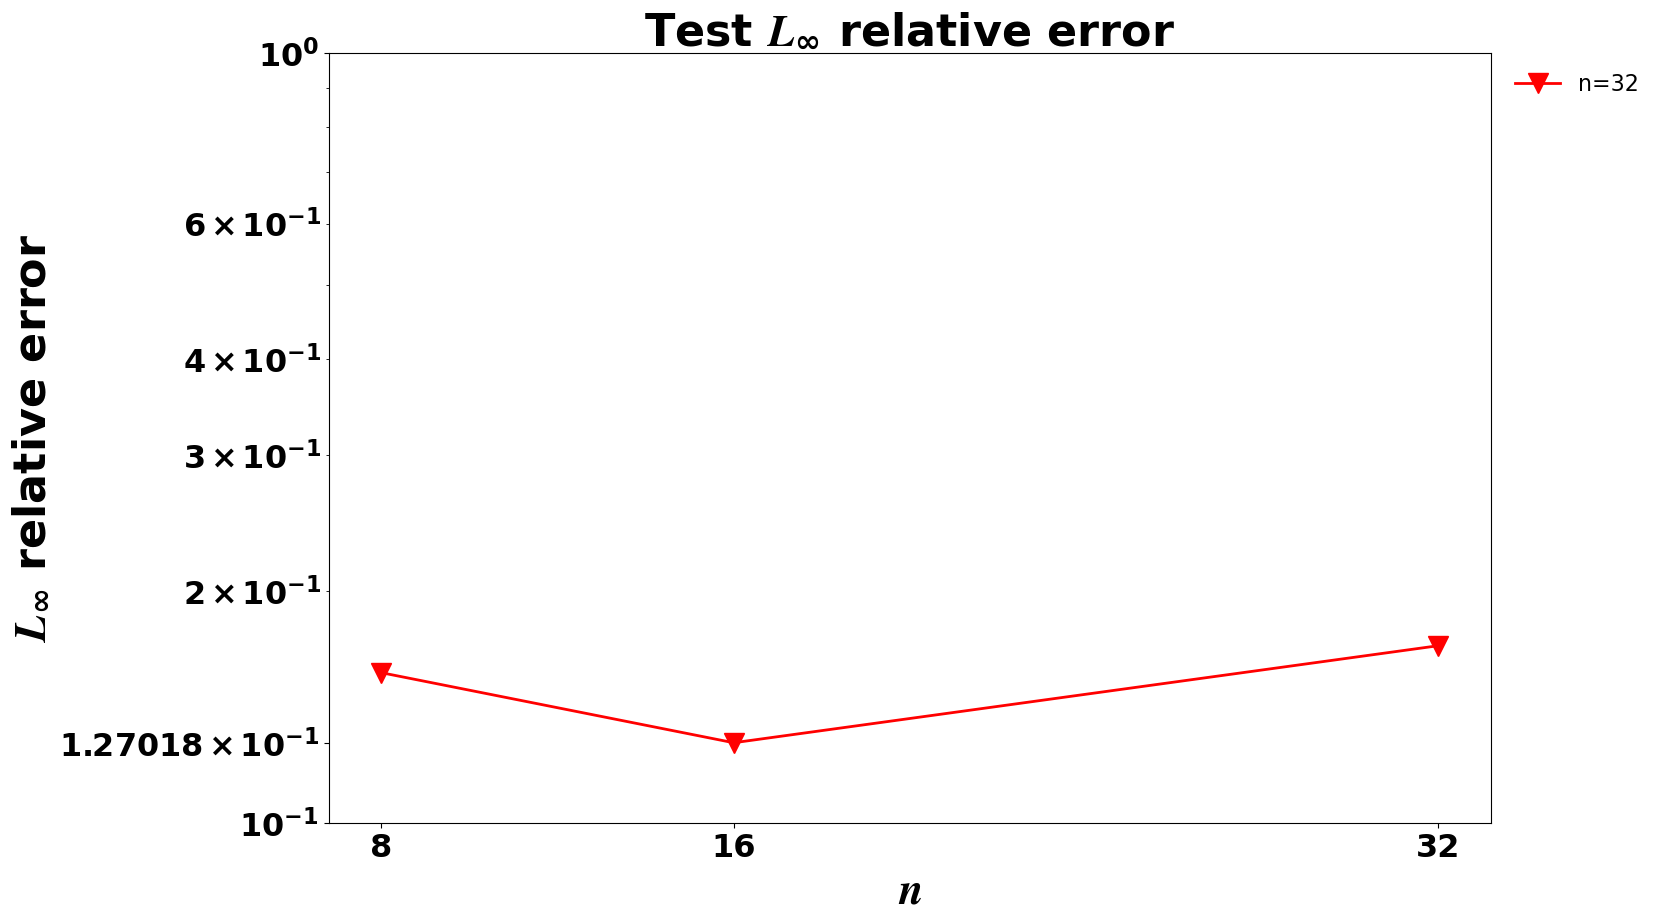
\includegraphics[width=0.5\linewidth]{all_plots/Advection/test_linf_vs_size.png} 
    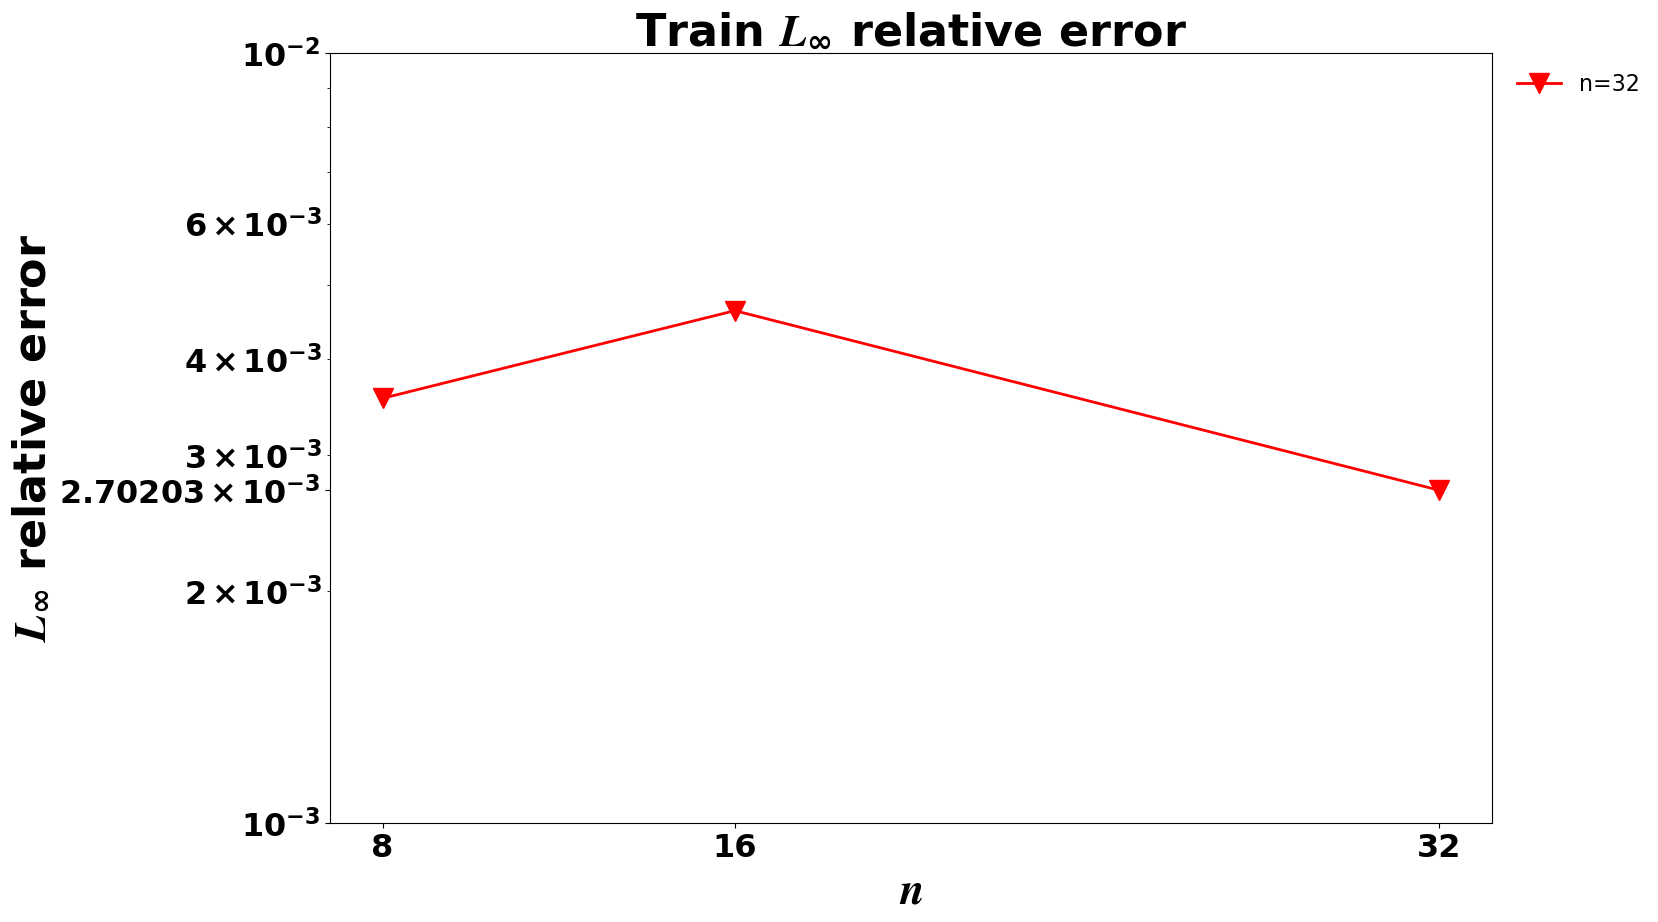
\includegraphics[width=0.5\linewidth]{all_plots/Advection/train_linf_vs_size.png} 
    \caption{Relative $L_\infty$ errors on the training and test sets for the Advection equation.}
    \label{fig:advection_linf}
\end{figure}

Figures \ref{fig:advection_l2} and \ref{fig:advection_linf} show the relative errors on the Advection equation. We see similar VANO perform similarly in this problem as well. Since the problem is one-dimensional, the errors remain constant w.r.t. increasing $n$. We also observe a generally better order of error in this problem, $1e-3$. Further experiments are required to push the VANO error down further on space-time problems, potentially with a different encoding for the temporal component.

\item Darcy flow

\begin{figure}[h]
    \centering
    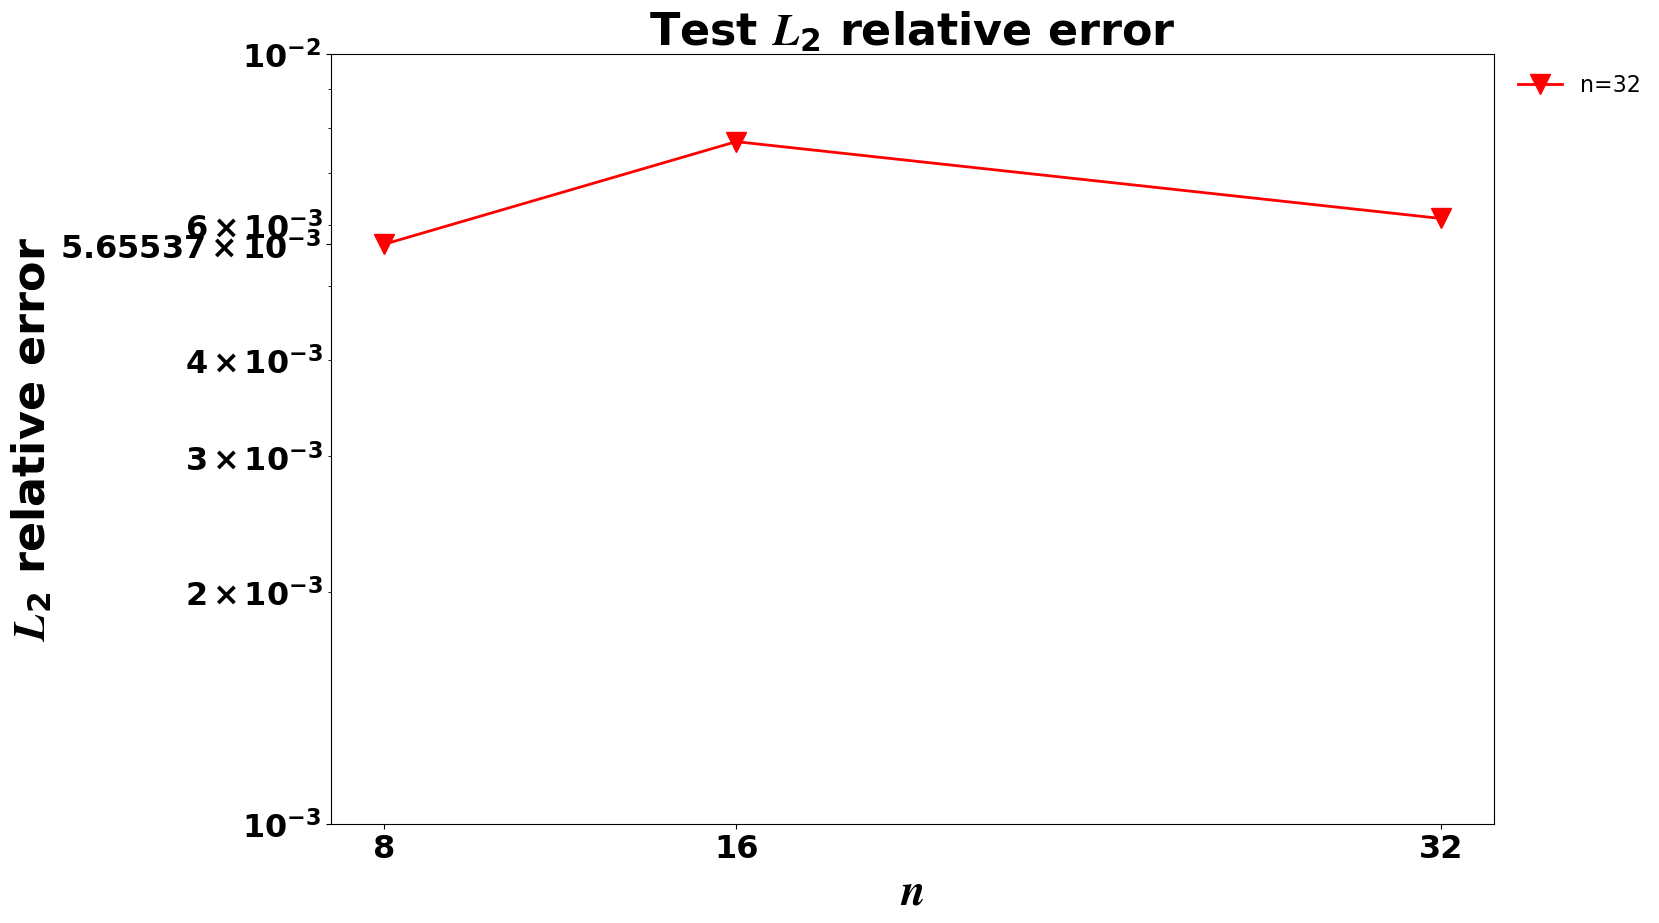
\includegraphics[width=0.5\linewidth]{all_plots/Darcy_triangular/test_l2_vs_size.png} 
    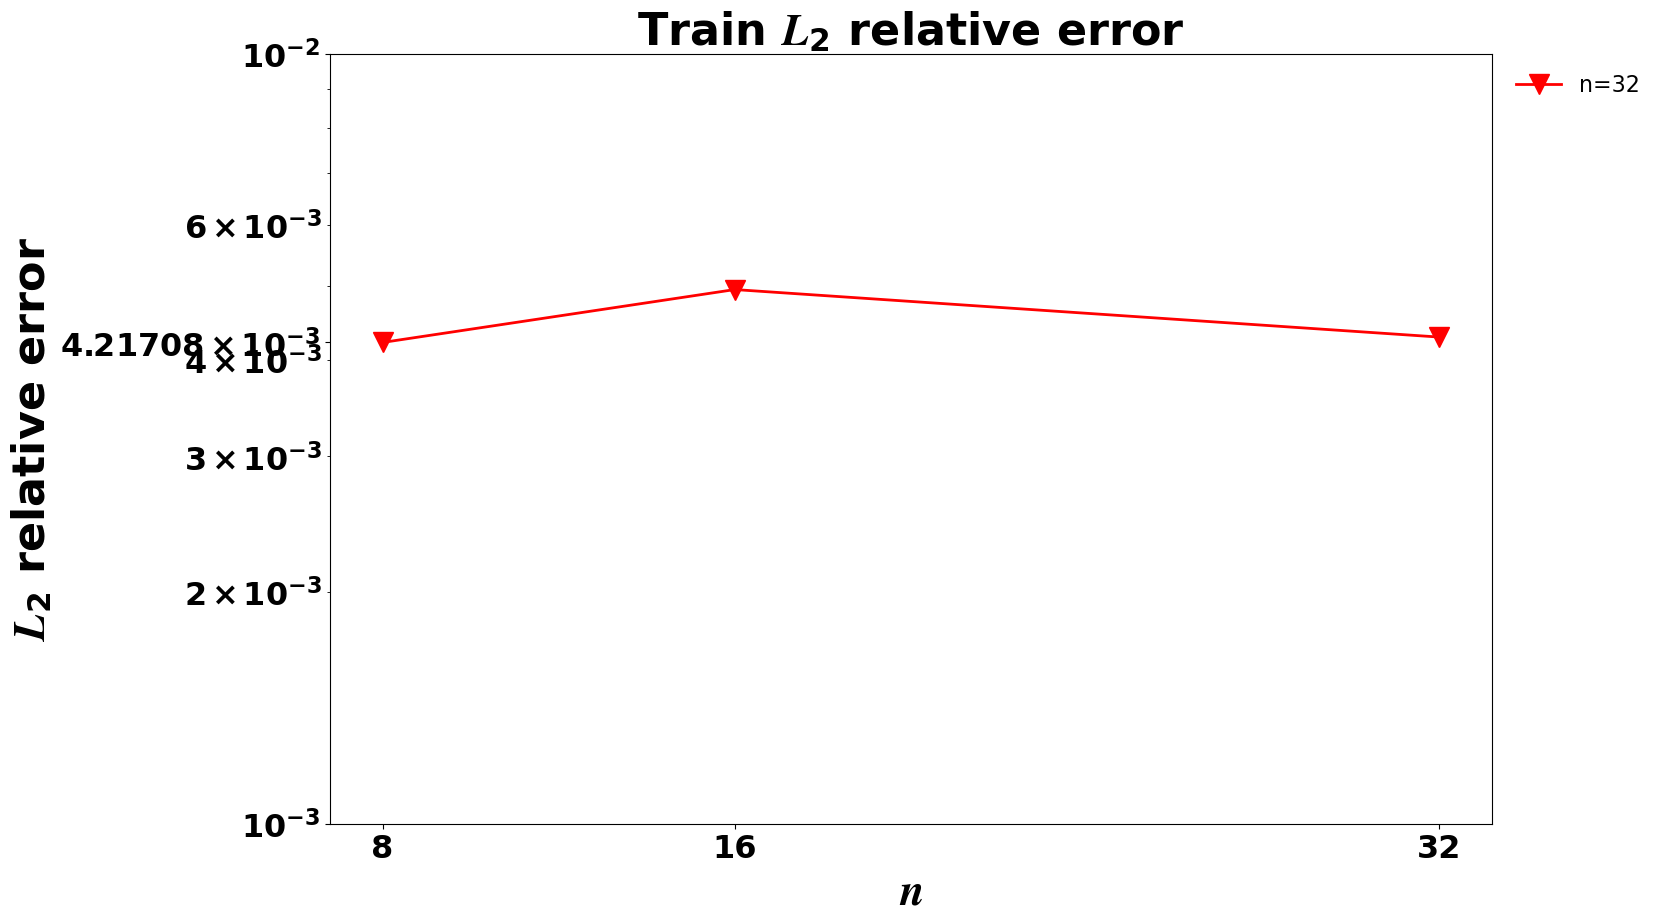
\includegraphics[width=0.5\linewidth]{all_plots/Darcy_triangular/train_l2_vs_size.png} 
    \caption{Relative $L_2$ errors on the training and test sets for the Darcy flow equation on the triangular domain.}
    \label{fig:darcy_tri_l2}
\end{figure}

\begin{figure}[h]
    \centering
    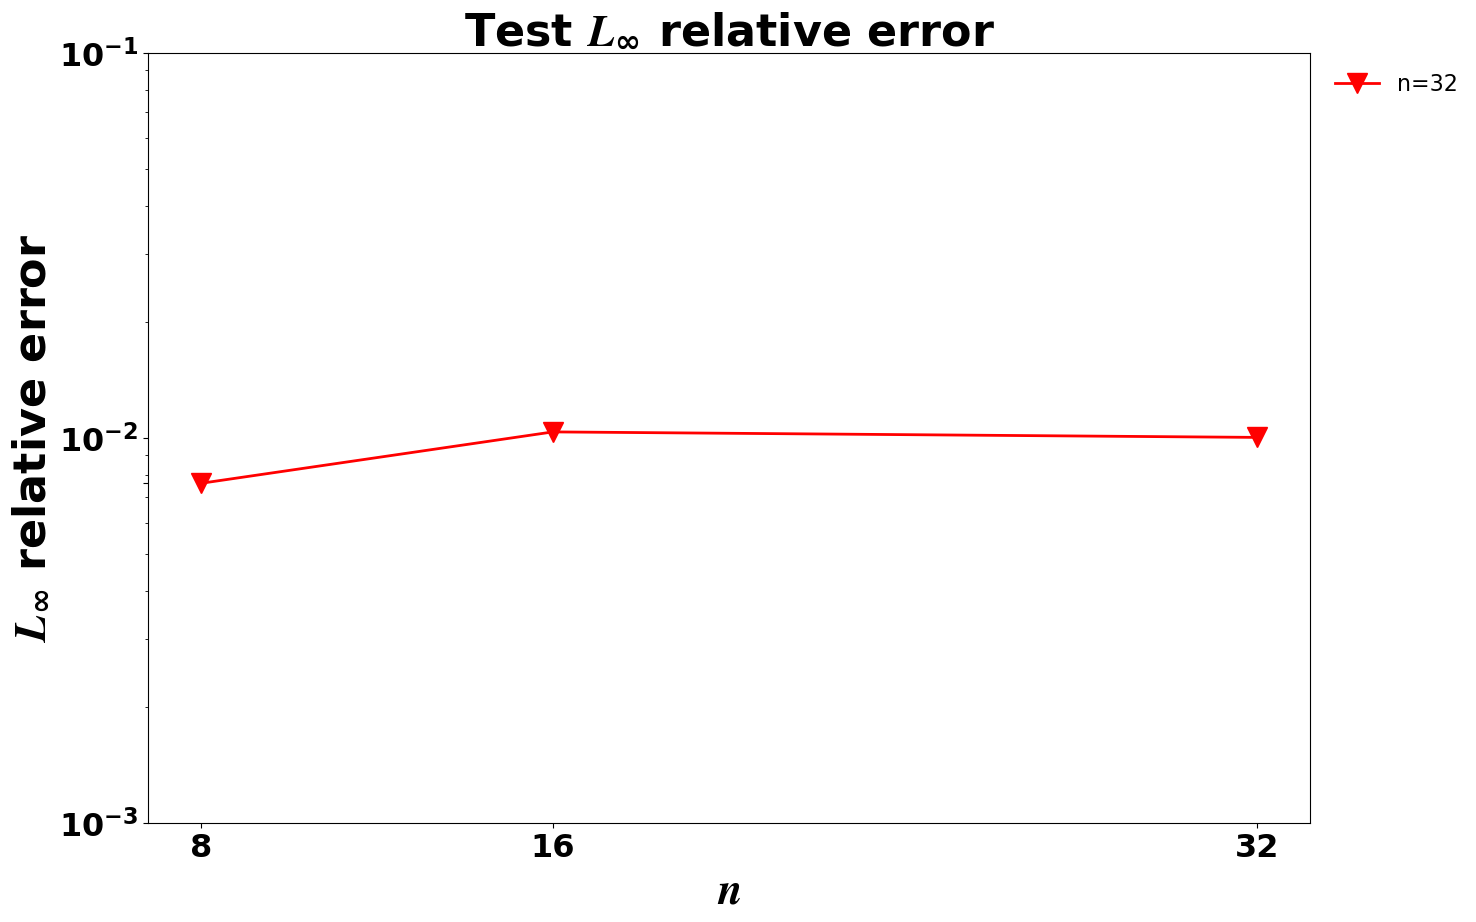
\includegraphics[width=0.5\linewidth]{all_plots/Darcy_triangular/test_linf_vs_size.png} 
    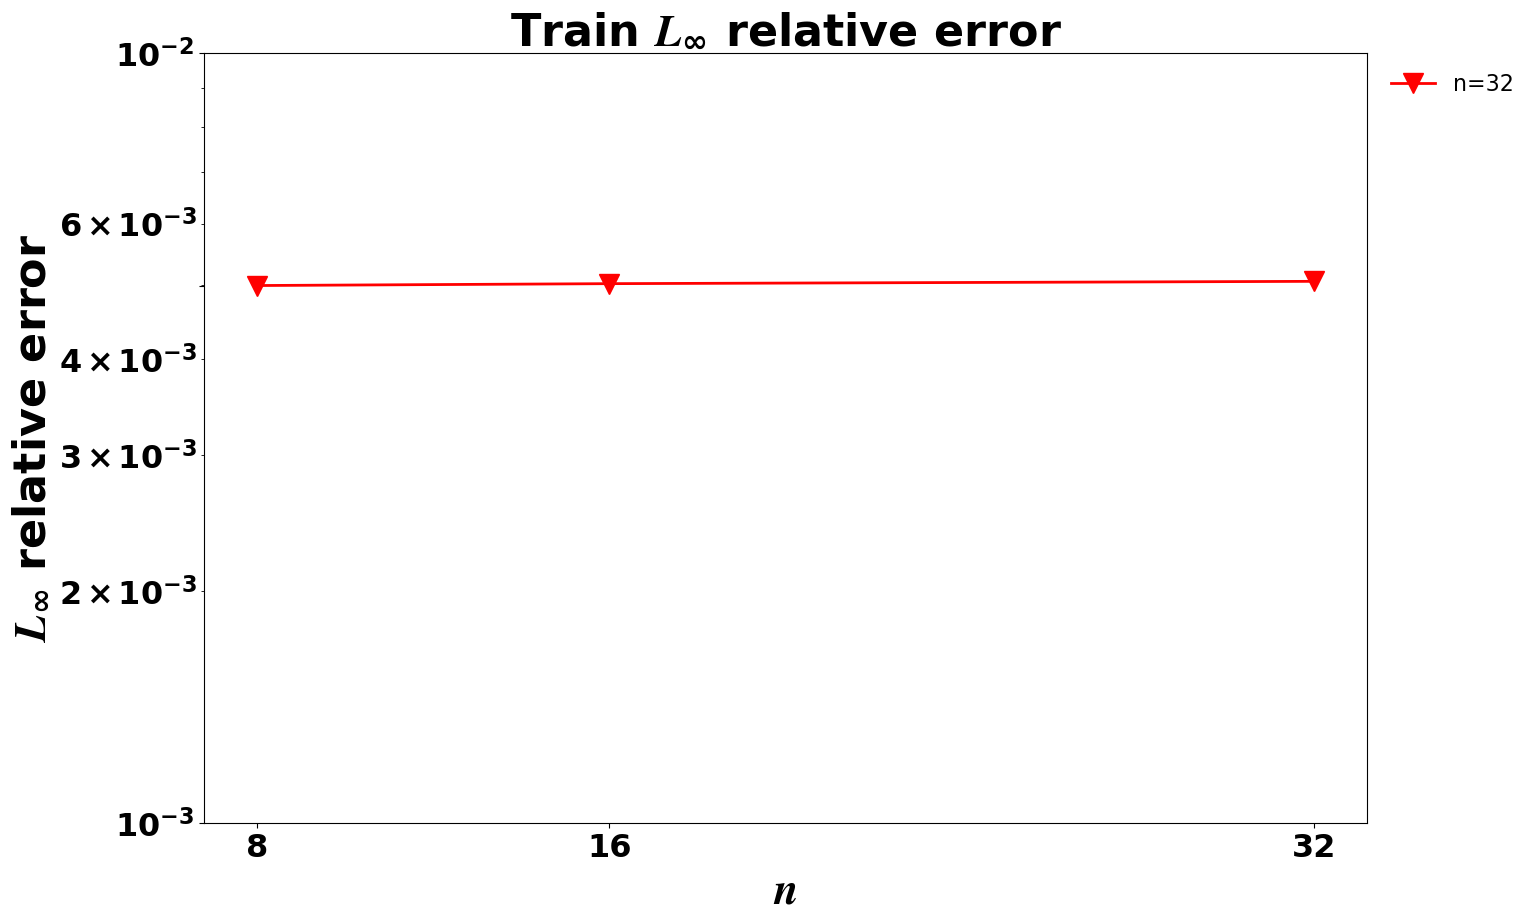
\includegraphics[width=0.5\linewidth]{all_plots/Darcy_triangular/train_linf_vs_size.png} 
    \caption{Relative $L_\infty$ errors on the training and test sets for the Darcy flow equation on the triangular domain.}
    \label{fig:darcy_tri_linf}
\end{figure}

Lastly, Figures \ref{fig:darcy_tri_l2} and \ref{fig:darcy_tri_linf} show the relative errors on the Darcy flow problem on a triangular domain. While the order of error in this problem also goes down sufficiently low, $1e-3$, we observe that increasing $n$ does not decrease the errors on either the training or test sets. Therefore, either a richer latent representation of the input functions is unnecessary in the given datasets, or a different VANO architecture is required to capture more spatial information. One way to improve the encoder architecture in this regard is to use other standard networks (CNNs, graph neural networks) to encode spatial information better. We leave this for future experiments on these datasets.

\end{enumerate}



\section{Conclusion and Future Work}
% other genrative models for functional data, 

In the future, the important next step for VANOs is to apply the model to learn PDE operators and functional mappings other than the identity operator. Neither this work nor the original authors have done this as far as we know. We emphasize the ability of this model to learn the identity operator on functional data should not be understated because it implies a very useful capability. This is because functions are agnostic of their discretization in general, and accordingly, VANO can be used on datasets of any resolution (by using a set of evaluation points in the decoder MLP different from the points used in the input function evaluation). In particular, images can be thought of as functions and thus VANO provides an ability to train generative models that aren't particular to image resolutions. We imagine many different generative models will be adapted to work on functional data in the future with this methodology such as diffusion models and normalizing flows. In fact, recent papers on these subjects are tangentially approaching this idea \cite{meng2023variational}.

\bibliographystyle{siam}
\bibliography{ref}
\end{document}
\endinput
